\documentclass[10pt,a4paper]{article}
\usepackage[a4paper]{geometry}

\usepackage{polski}
\usepackage{indentfirst}
\usepackage{xltxtra}
\usepackage{relsize}
\usepackage{fancyvrb}
\usepackage[pdfborder={0 0 0}]{hyperref}
\usepackage{graphicx}
\usepackage{changepage}

\defaultfontfeatures{Mapping=tex-text}
\setromanfont{Charis SIL}
\setmonofont[Scale=MatchLowercase]{Menlo}
\linespread{1.25}

\DefineVerbatimEnvironment%
  {SmallVerbatim}%
  {Verbatim}{fontsize=\relsize{-0.5},numbers=left,numbersep=-10pt,frame=lines,tabsize=4}

\newcommand{\f}[1]{\texttt{#1}}

\begin{document}

%%fakesection{Tytuł}
\title{ 
  Interpolacja funkcjami sklejanymi\\
  {\normalsize Specyfikacja implementacyjna projektu nr 2}\\\vspace{-12pt}
  {\normalsize z przedmiotu \emph{Języki i metody programowania 2}}
}
\author{
  Tomasz Cudziło\\
  {\small EE PW, 211552}
}
\date{\today}
\maketitle

\section*{Zadanie}
\label{sec:zadanie}

Napisać program, z~graficznym interfejsem użytkownika, wyznaczający
współczynniki funkcji sklejanych trzeciego stopnia aproksymujących zadany ciąg
danych pomiarowych.

\vspace{20pt}

\section{Logika klas}

Cały projekt jest luźno oparty na wzorcu \f{MVC}. Punktem wejścia jest klasa
\f{SplinesApp}, która posiada obiekt klasy \f{SplinesController}. Ta
instancja kontrolera, posiada obiekty punktów, wielomianów i~wykres, oraz
zarządza nimi zgodnie z~poleceniami użytkownika płynącymi z~instancji
\f{SplinesView}.

Schemat z~rys.~\ref{fig:aplikacja} na stronie \pageref{fig:aplikacja}
przedstawia zarys podziału problemu na klasy.

\newpage
\begin{figure}[ht]
  \begin{adjustwidth}{-3cm}{-3cm}
    \centering
    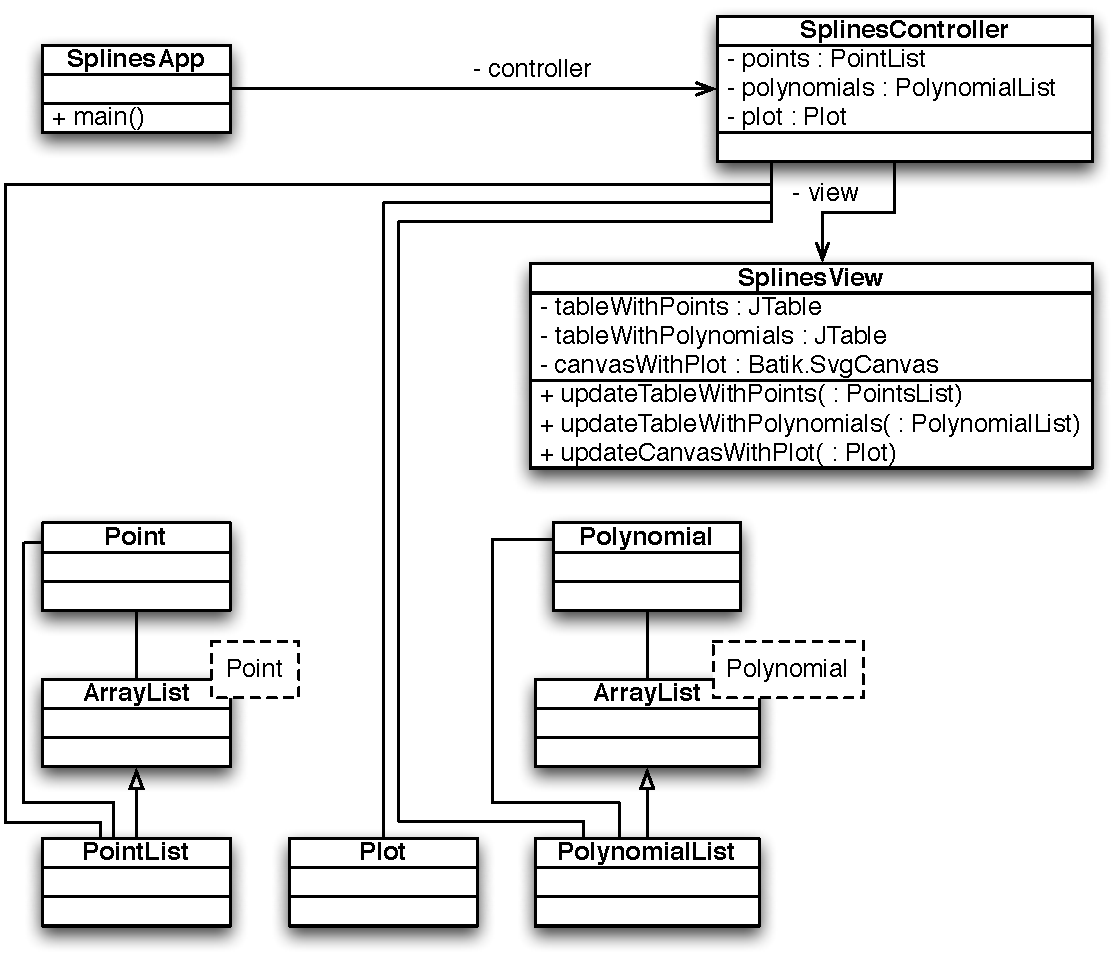
\includegraphics{figury/aplikacja}
    \caption{Schemat całej aplikacji.}
    \label{fig:aplikacja}
  \end{adjustwidth}
\end{figure}
\clearpage

\subsection{Aplikacja}

Klasa \f{SplinesApp} (rys. \ref{fig:aplikacja-szczegolowo}) jest punktem
wejściowym programu. Jednocześnie jest zaimplementowana jako \f{Singleton},
który służy do wywoływania binarki z~pierwszego projektu.

Metoda \f{main()} inicjuje stan \f{SplinesApp}, to znaczy sprawdza czy
\f{splines} jest widoczne z~\f{PATH}, i~zapamiętuje ścieżkę. Następnie tworzy
i~uruchamia \f{SplinesController}.

Klasa udostępnia metody zwracające dane wygenerowane przez binarkę z~pierwszego
projektu.

\begin{figure}[hb]
  \centering
  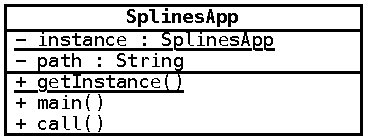
\includegraphics{figury/aplikacja-szczegolowo}
  \caption{Schemat \f{SplinesApp}.}
  \label{fig:aplikacja-szczegolowo}
\end{figure}

\subsection{Modele}

\subsubsection{Punkty i~wielomiany}

Modele \f{PointList} i~\f{PolynomialList}\footnote{\f{PolynomialList} nie jest
modelem, wielomiany są zależne od punktów, ale dla wygody traktuję je jak
model.} zachowują się podobnie. Obydwa są tylko nakładkami na kolekcję
\f{ArrayList} przechowującą odpowiedni typ. Mają przeciążone metody
\f{toString()}, które zwracają całą kolekcję w~\f{String} w~formacie
odpowiednim dla plików tworzonych przez program.

Schemat dla \f{PointList} jest na stronie \pageref{fig:punkty-szczegolowo}.
Relacje między klasami dla \f{PolynomialList} są analogiczne.

\begin{figure}[ht]
  \centering
  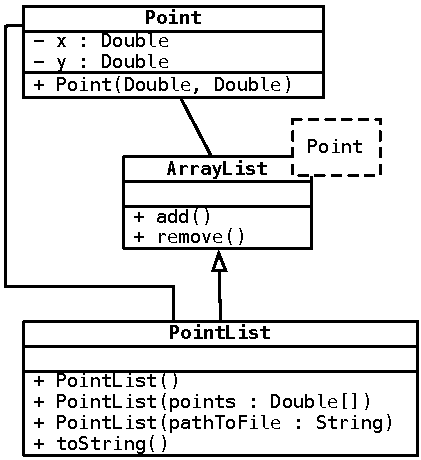
\includegraphics{figury/punkty-szczegolowo}
  \caption{Schemat klas odpowiadających za punkty.}
  \label{fig:punkty-szczegolowo}
\end{figure}

Klasy \f{Point} i~\f{Polynomial} są prostymi klasami zawierającymi tylko pola,
konstruktory zapełniające te pola oraz~przeciążone \f{toString()}. Jeśli będzie
to możliwe, zostaną one klasami wewnętrznymi zdefiniowanymi w~klasach \f{List}
im odpowiadającym.

\subsubsection{Wykres}

Podobnie jak \f{PolynomialList} klasa \f{Plot} nie jest modelem, ale traktuję
ją jako model. Klasa posiada metody pozwalające na eksport do różnych formatów,
które korzystają z~jednej ogólnej metody eksportującej.

\subsubsection{Generowanie wielomianów i~wykresu}

Zarówno wielomiany i~wykres są tworzone przez programy zewnętrzne \f{splines}
i~\f{gnuplot}. Tworzone są przez wywoływanie odpowiadających im metod klasy
\f{SplinesApp}.

\subsection{Kontroler}

Kontroler \f{SplinesController}, zarządza całym programem na wyższym poziomie
abstrakcji niż reszta klas. Jego jedynym zadaniem jest odpowiadanie na eventy
przychodzące z~\f{SplinesView}, to znaczy widok wywołuje odpowiednie metody
kontrolera, a~następnie kontroler wywołuje metody modeli.

Przykład komunikacji przy odświeżaniu wykresu znajduje się na schemacie
nr~\ref{fig:wykres-rysuj}.

\begin{figure}[ht]
  \begin{adjustwidth}{-2cm}{-2cm}
    \centering
    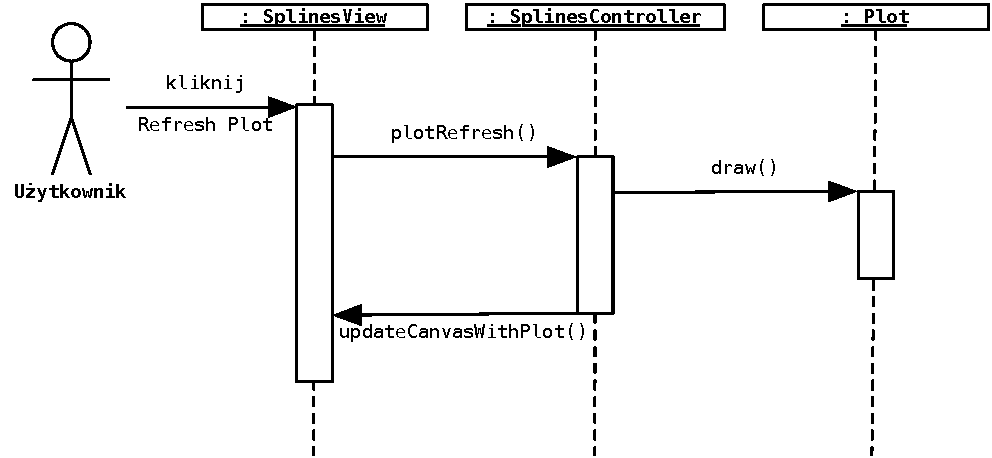
\includegraphics{figury/wykres-rysuj}
    \caption{Przykład interakcji między widokiem a~kontrolerem.}
    \label{fig:wykres-rysuj}
  \end{adjustwidth}
\end{figure}

\subsection{Widok}

\subsubsection{Okno główne}

Klasa \f{SplinesView} nie zawiera żadnej logiki. Tworzy tylko okno główne
aplikacji, a~wszystkie eventy od użytkownika są przekazywane do kontrolera.

Do konstrukcji okna wykorzystywane są elementy z~frameworku \f{Swing}. Drzewko
wykorzystanych elementów znajduje się na rys. \ref{fig:aplikacja-widok}
str.~\pageref{fig:aplikacja-widok}.

\subsubsection{Okno eksportu wykresu}

Okno eksportu wykresu dziedziczy po \f{JDialog} i~zawiera podstawowe kontrolki
z~pakietu \f{Swing}. Drzewo elementów na rys.~\ref{fig:wykres-rysuj-widok}. Jest
tworzone przez kontroler i~po zamknięciu zwraca mu wprowadzone wartości.

\begin{figure}[p]
  \centering
  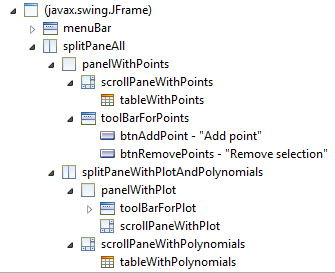
\includegraphics[width=0.67\textwidth]{figury/aplikacja-widok}
  \caption{Drzewo elementów tworzących okno główne aplikacji.}
  \label{fig:aplikacja-widok}
\end{figure}

\begin{figure}[p]
  \centering
  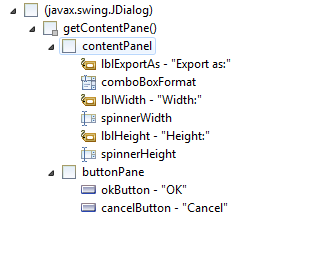
\includegraphics[width=0.67\textwidth]{figury/wykres-rysuj-widok}
  \caption{Drzewo elementów tworzących okno pomocnicze eksportu wykresu.}
  \label{fig:wykres-rysuj-widok}
\end{figure}

\section{Pliki}

\end{document}
